\section{ Applying Linear Combination to Limits }

\displaytwocaption{Results of Using Linear Combination for Limits}{
    The new combination currently retains VHH contamination, but that will be removed soon.
    Otherwise, limits show good agreement with 3-term-based results.
}{c2v_scan_official}{Original 3 Term Combination}
{c2v_scan_new_kl1.0}{New 6 Term Combination}


\displaythree{$\kvv$ Scans Outside $\kl=1$}
{ Linear combination equation seems to work well beyond the SM value of $\kl$ }
{c2v_scan_scan_test_beta5_samps_vbf_pd_161718_kl1.0_xsec}
{c2v_scan_scan_test_beta5_samps_vbf_pd_161718_kl3.0_xsec}
{c2v_scan_scan_test_beta5_samps_vbf_pd_161718_kl7.0_xsec}

\frame{
    \frametitle{Visualizing Exclusion Zones} 
    \begin{columns}
        \begin{column}{0.5\textwidth}
            \begin{figure}
                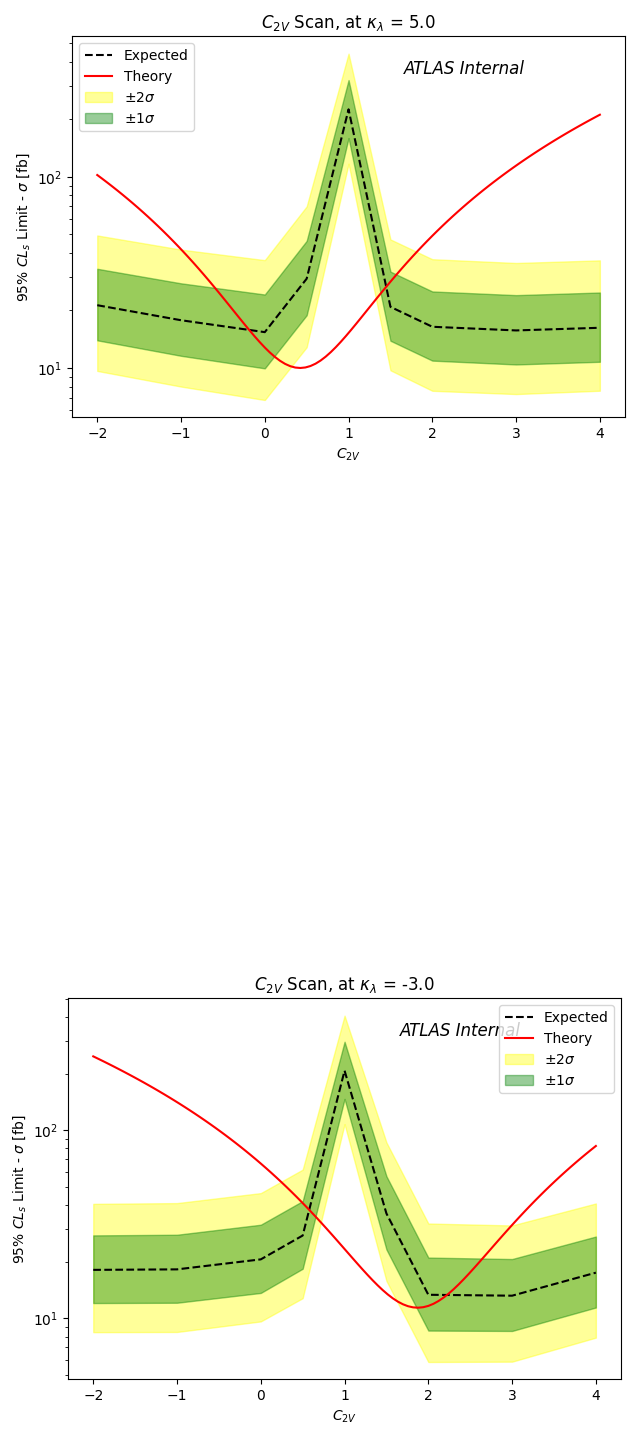
\includegraphics[width=\linewidth,height=0.8\textheight,keepaspectratio]{2D_explanation00}
            \end{figure}
        \end{column}
        \begin{column}{0.5\textwidth}
            It would be nice to see more than a couple values of $\kl$ at a time...
        \end{column}
    \end{columns}
}

\frame{
    \frametitle{Visualizing Exclusion Zones} 
    \begin{columns}
        \begin{column}{0.5\textwidth}
            \begin{figure}
                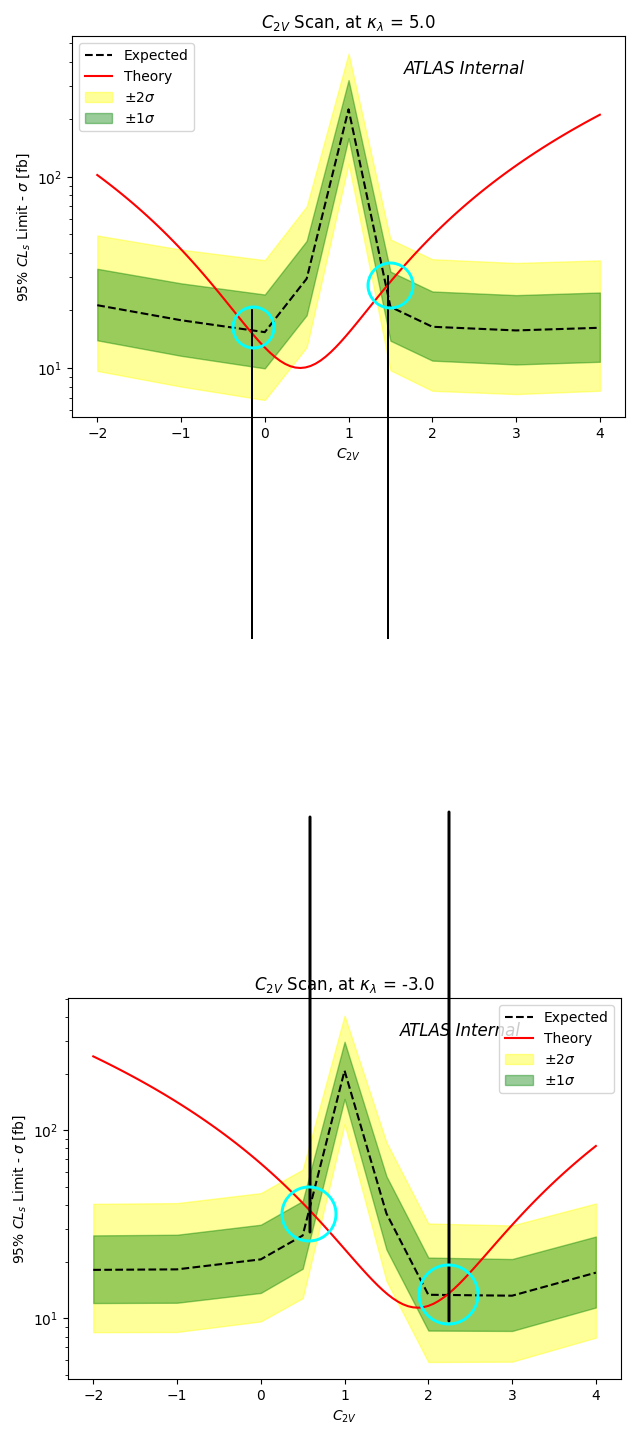
\includegraphics[width=\linewidth,height=0.8\textheight,keepaspectratio]{2D_explanation01}
            \end{figure}
        \end{column}
        \begin{column}{0.5\textwidth}
            Exclusion is denoted by the point at which the theory and expectation lines cross.
        \end{column}
    \end{columns}
}

\frame{
    \frametitle{Visualizing Exclusion Zones} 
    \begin{columns}
        \begin{column}{0.5\textwidth}
            \begin{figure}
                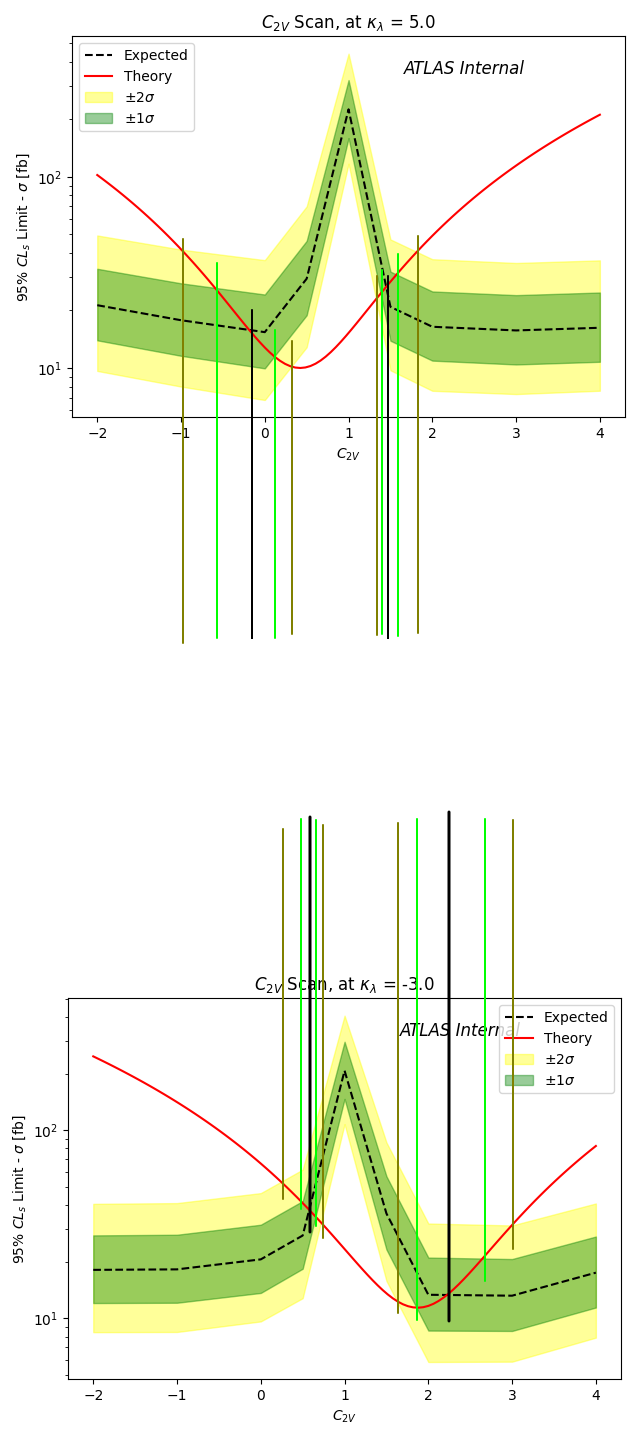
\includegraphics[width=\linewidth,height=0.8\textheight,keepaspectratio]{2D_explanation02}
            \end{figure}
        \end{column}
        \begin{column}{0.5\textwidth}
            Exclusion to 1 and 2 sigma can be similarly be found
        \end{column}
    \end{columns}
}

\frame{
    \frametitle{Visualizing Exclusion Zones} 
    \begin{columns}
        \begin{column}{0.5\textwidth}
            \begin{figure}
                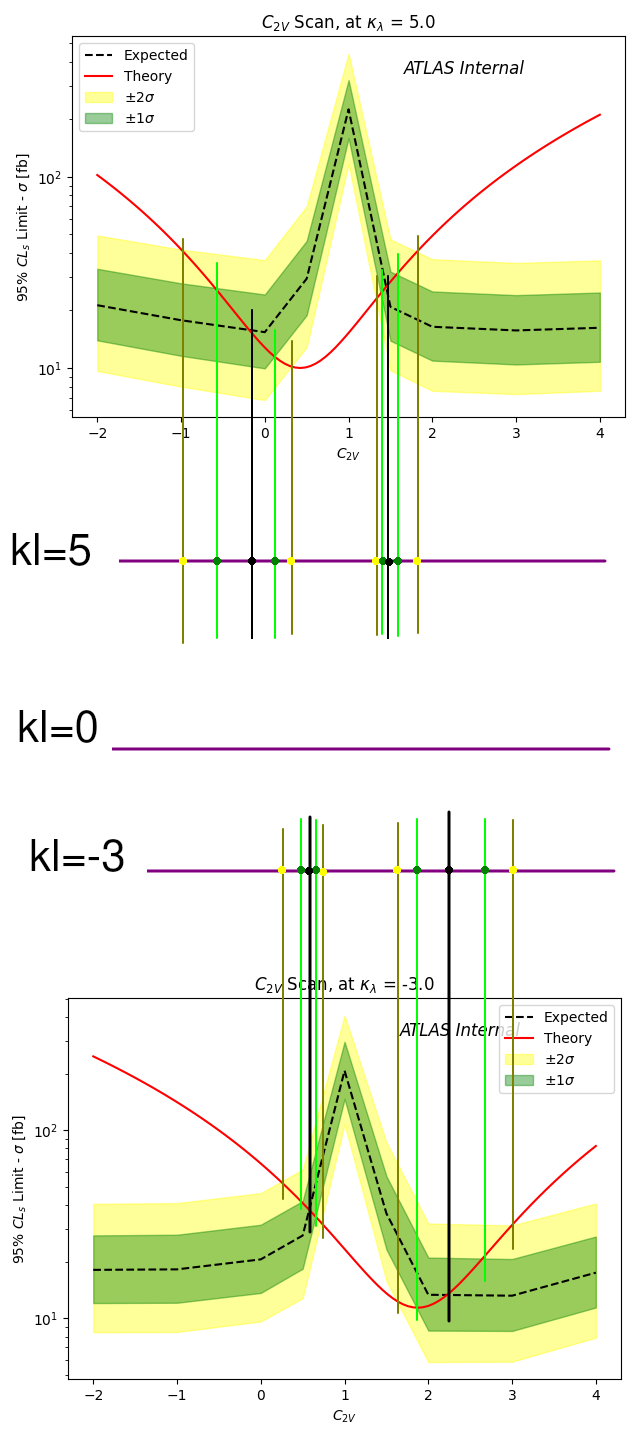
\includegraphics[width=\linewidth,height=0.8\textheight,keepaspectratio]{2D_explanation03}
            \end{figure}
        \end{column}
        \begin{column}{0.5\textwidth}
            All these intersections can be represented as points in $\kl$ space.
        \end{column}
    \end{columns}
}

\frame{
    \frametitle{Visualizing Exclusion Zones} 
    \begin{columns}
        \begin{column}{0.5\textwidth}
            \begin{figure}
                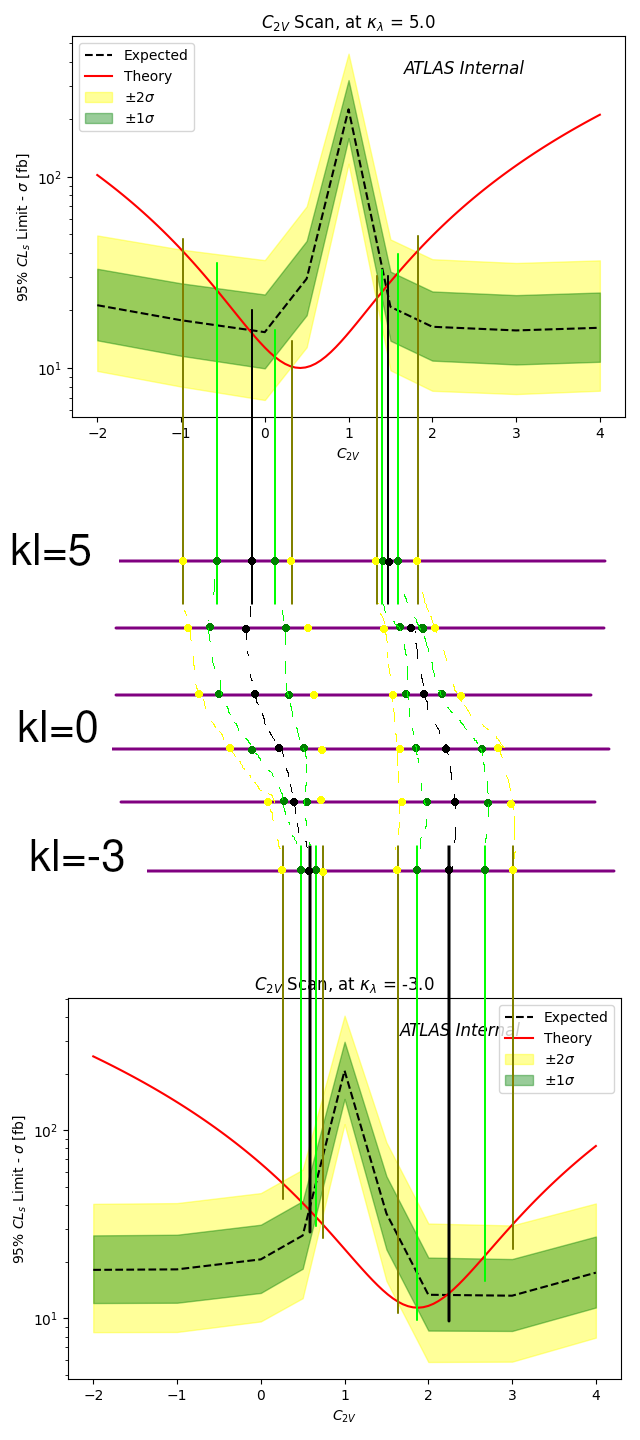
\includegraphics[width=\linewidth,height=0.8\textheight,keepaspectratio]{2D_explanation04}
            \end{figure}
        \end{column}
        \begin{column}{0.5\textwidth}
            Connect many such intersections in $\kl$ and $\kvv$ space through interpolation to obtain...
        \end{column}
    \end{columns}
}

\frame{
    \frametitle{Visualizing Exclusion Zones} 
    \begin{columns}
        \begin{column}{0.5\textwidth}
            \begin{figure}
                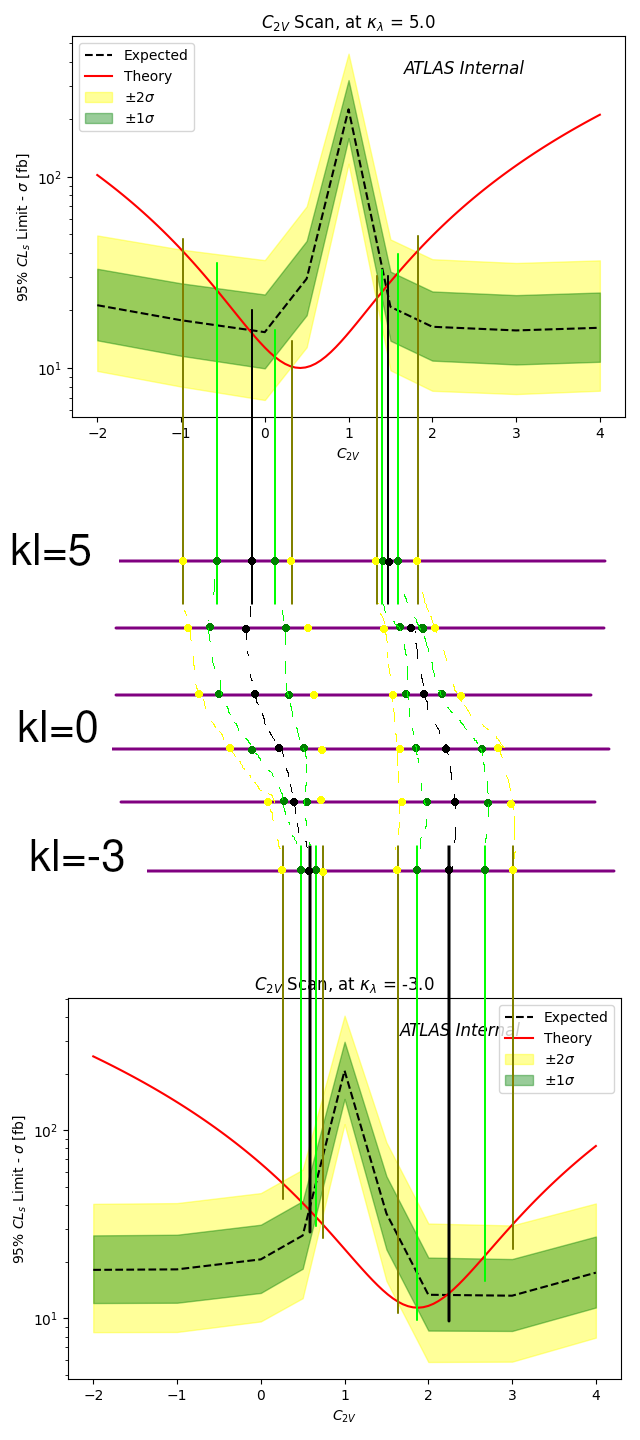
\includegraphics[width=\linewidth,height=0.8\textheight,keepaspectratio]{2D_explanation04}
            \end{figure}
        \end{column}
        \begin{column}{0.5\textwidth}
                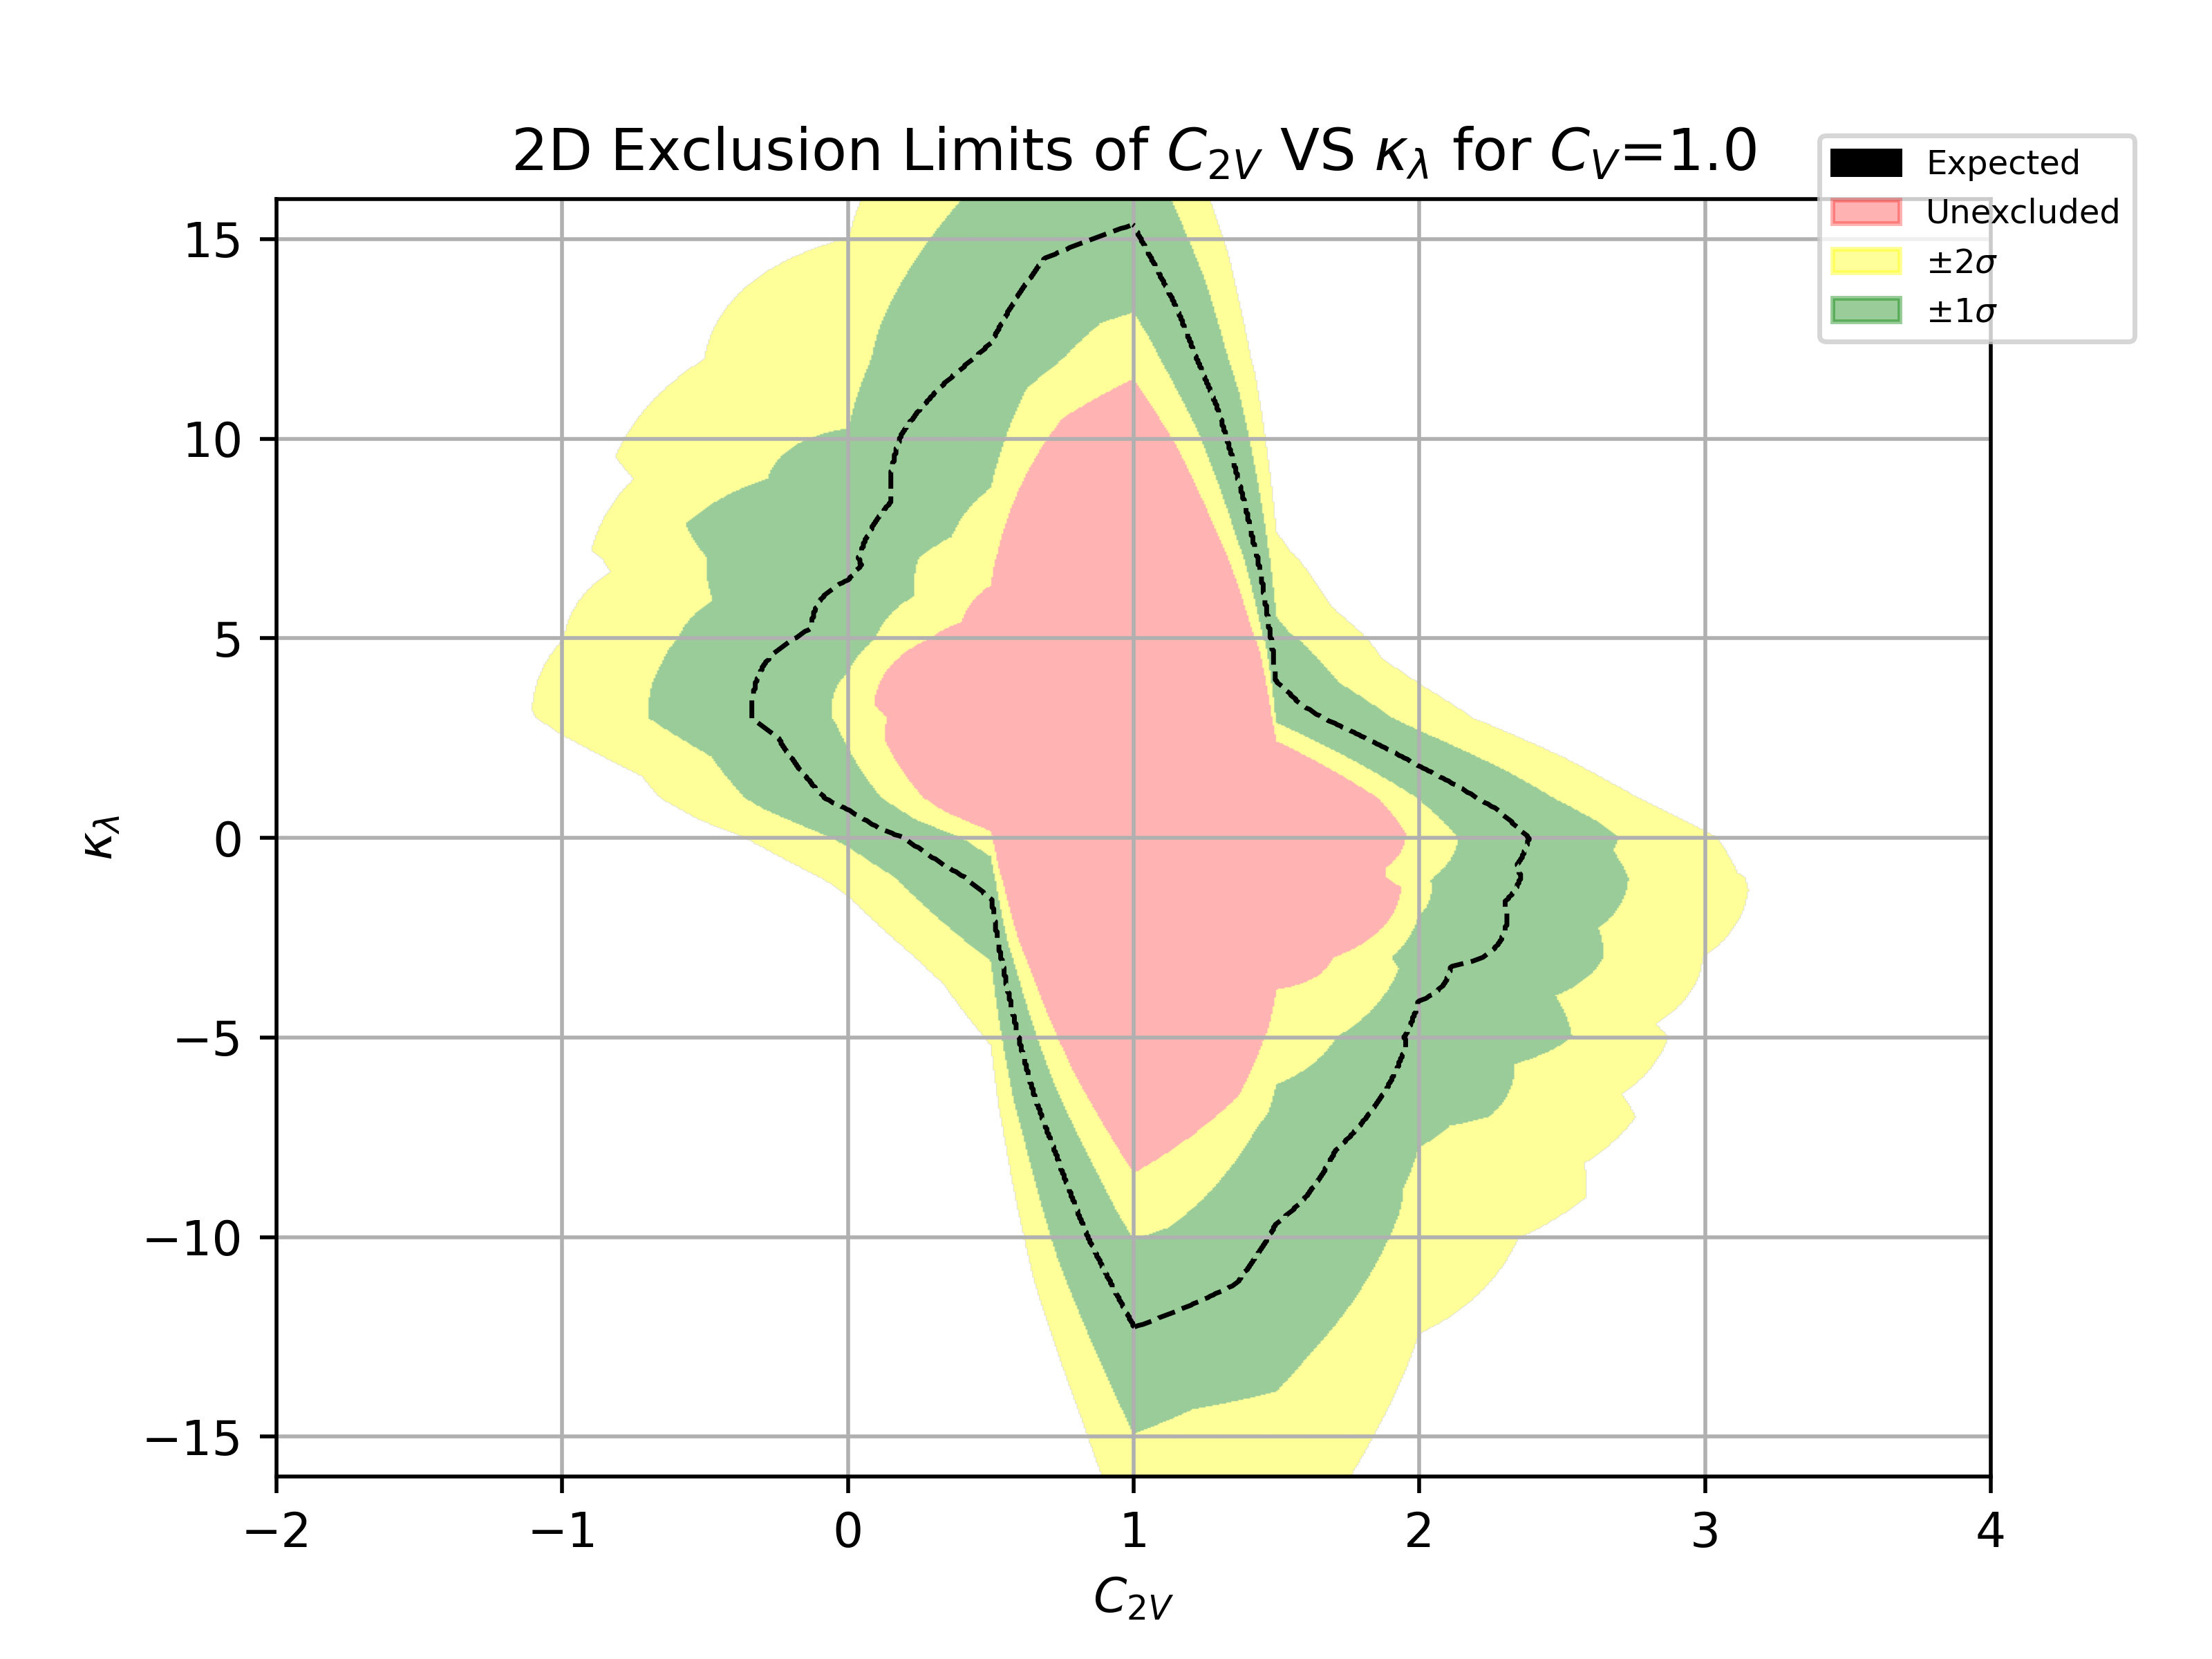
\includegraphics[width=\linewidth,height=0.8\textheight,keepaspectratio]{2D_scan_scan_test_beta5_samps_vbf_pd_161718_c1v1.0_exclusion}
        \end{column}
    \end{columns}
}

\fullscreenimage{Exclusion Across 3D Parameter Space}
{2D_scan_scan_test_beta5_samps_vbf_pd_161718_c1v_multislice_exclusion}

\fullscreenimage{Exclusion From a Different Perspective}
{2D_scan_scan_test_beta5_samps_vbf_pd_161718_kl_multislice_exclusion}

\fullscreenimage{For the Sake of Completeness}
{2D_scan_scan_test_beta5_samps_vbf_pd_161718_c2v_multislice_exclusion}
